$l$ and $m$ are two parallel lines intersected by another pair of parallel lines $p$ and $q (\figref{fig:fig:1})$,show that $\triangle ABC \cong \triangle CDA$.


\textbf{Figure :}
\begin{figure}[H]
    \centering
	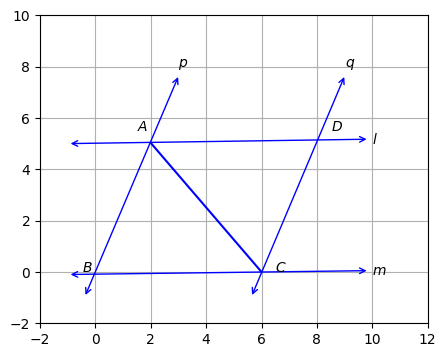
\includegraphics[width=\columnwidth]{chapters/9/7/1/4/fig/em1.png}
    \caption{Required parallelogram}
    \label{fig:fig:1}
\end{figure}
\textbf{Solution :}\\
\begin{table}[h]
    \centering
	  \begin{tabular}{|c|c|c|}
    \hline
        \textbf{Symbol} &\textbf{Description}&\textbf{Value}  \\
        \hline
        $\vec{B}$&Vertex at origin&$\vec{0}$\\
        \hline
        $a$ & Side of the parallelogram,$BC=DA$ & 6\\
        \hline
        $b$ & Side of the parallelogram,$AB=CD$& $\sqrt{29}$\\
        \hline
        $\theta$ & Angle of the parallelogram, $\angle ABC$& $\sin^{-1}\brak{{\frac{5}{\sqrt{29}}}}$\\
        \hline
    \end{tabular}

    \caption{Table of input parameters}
    \label{tab:tab:1}
\end{table}
\begin{table}[h]
    \centering
       \begin{tabular}{|c|c|c|}
    \hline
        \textbf{Symbol} &\textbf{Description}&\textbf{Value}  \\
        \hline
	   $\vec{C}$&Vertex of parallelogram &$a\vec{e_1}$\\
        \hline
         $\vec{A}$&Vertex of parallelogram &$b\begin{pmatrix}
             \cos{\theta}\\
             \sin{\theta}
         \end{pmatrix}$\\
        \hline
        $\vec{D}$&Vertex of parallelogram &$\vec{C+A}$\\
        \hline
    \end{tabular}

    \caption{Table of output parameters}
    \label{tab:tab:2}
\end{table} 


From $\figref{fig:fig:1}$ between $\triangle ABC $ and $\triangle CDA$
\begin{align}
\cos{\angle BAC} &= \frac{AB.CA}{\norm{AB}\norm{CA}}\\
&=\frac{ab\cos{\theta}+b\sin{\theta}}{b\sqrt{a^2-2ab\cos{\theta}+b^2}}\\
&=\frac{17}{\sqrt{29}\sqrt{41}}\\
\cos{\angle ACD} &= \frac{CD.CA}{\norm{CD}\norm{CA}}\\
&= \frac{b^2-ab\cos{\theta}}{b\sqrt{a^2-2ab\cos{\theta}+b^2}}\\
&=\frac{17}{\sqrt{29}\sqrt{41}}\\
So,\angle BAC = \angle ACD.\\
\cos{\angle ACB} &= \frac{CB.CA}{\norm{CB}\norm{CA}}\\
&=\frac{a^2-ab\cos{\theta}}{a\sqrt{a^2-2ab\cos{\theta}+b^2}}\\
&=\frac{24}{6\sqrt{41}}\\
\cos{\angle} CAD &= \frac{DA.CA}{\norm{DA}\norm{CA}}\\
&=\frac{a^2-ab\cos{\theta}}{a\sqrt{a^2-2ab\cos{\theta}+b^2}}\\
&=\frac{24}{6\sqrt{41}}\\
So,\angle ACB = \angle CAD.
\end{align}
And $CA$ is common side .

So,$\triangle ABC \cong \triangle CDA.\brak{by A-A-S}\brak{proved}$


